%%%%%%%%%%%%%%%%%%%%%%%%%%%%%%%%%%%%%%%%%%%%%%%%%%%%%%%%%%%%%%%%%%%%%%%%%%%%%%%
% Appendix B - Accessing the DMD on the DLP LightCrafter
%%%%%%%%%%%%%%%%%%%%%%%%%%%%%%%%%%%%%%%%%%%%%%%%%%%%%%%%%%%%%%%%%%%%%%%%%%%%%%%

\chapter{Accessing the DMD on the DLP LightCrafter}

The Texas Instruments DLP LightCrafter evaluation module contains a DLP3000 DMD, a DM365 embedded processor running Linux, and an RGB LED light engine developed by Young Optics (Figure \ref{fig:dmd_mod_0}). In order to utilize a custom light source such as a laser, the light engine must be removed to gain physical access to the DMD. The following series of figures details the disassembly process necessary to access and remount the DMD for use with custom illumination.

% Figure - LightCrafter Overview
\begin{figure}
    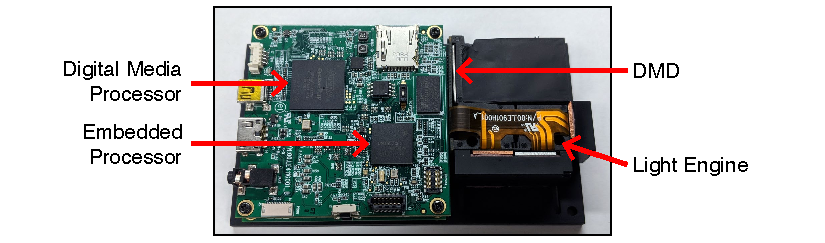
\includegraphics{figures/appendix_b/dmd_mod_0.pdf}
    \caption {
        \label{fig:dmd_mod_0}
        Overview of the Texas Instruments DLP LightCrafter.
    }
\end{figure}

Remove the four screws (Phillips head) on the top of device and detach the upper circuit board from the lower half of the device (Figure \ref{fig:dmd_mod_1}). Turn the device upside down and remove the four screws (Phillips head) attaching the light engine to the baseplate from the bottom (Figure \ref{fig:dmd_mod_2}). Flip the device back over and remove the three screws (Phillips head) attaching the light engine from the top. Remove the two screws (Phillips head) horizontally securing the light engine to the circuit board (Figure \ref{fig:dmd_mod_3}). Use a flat-head screwdriver to flip the locking clips on the two ribbon cables connecting the light engine to the circuit board and disconnect the cables.

% Figure - LightCrafter Modification: Step 1
\begin{figure}
    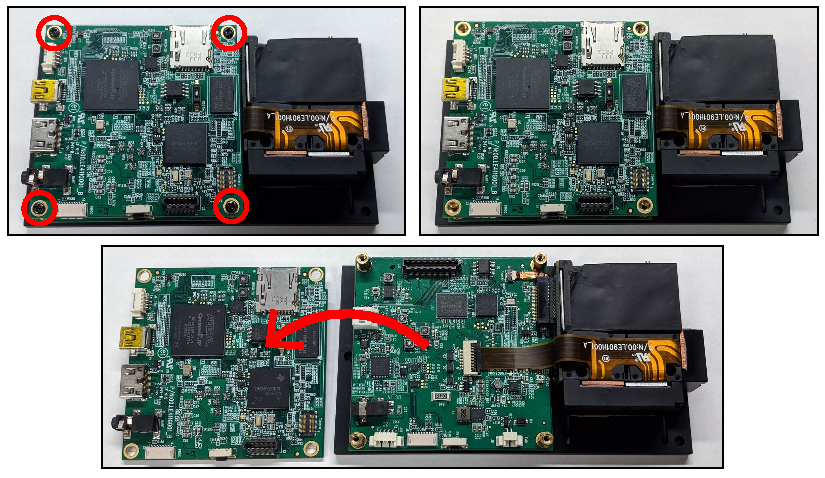
\includegraphics{figures/appendix_b/dmd_mod_1.pdf}
    \caption {
        \label{fig:dmd_mod_1}
        Detach the upper circuit board from the device.
    }
\end{figure}

% Figure - LightCrafter Modification: Step 2
\begin{figure}
    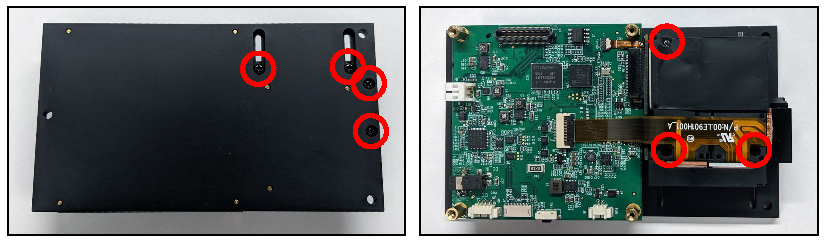
\includegraphics{figures/appendix_b/dmd_mod_2.pdf}
    \caption {
        \label{fig:dmd_mod_2}
        Remove the screws attaching the light engine to the baseplate.
    }
\end{figure}

% Figure - LightCrafter Modification: Step 3
\begin{figure}
    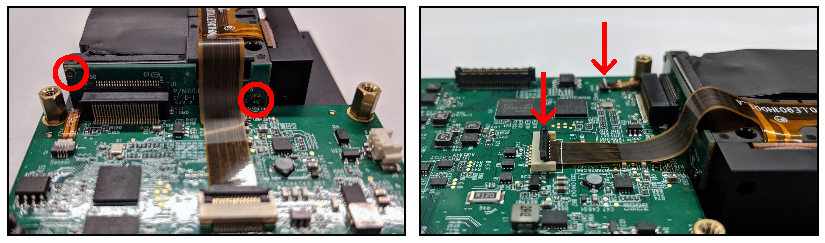
\includegraphics{figures/appendix_b/dmd_mod_3.pdf}
    \caption {
        \label{fig:dmd_mod_3}
        Remove the screws and ribbon cables connecting the light engine to the circuit board.
    }
\end{figure}

At this point, the only physical connection remaining between the light engine and the rest of the device is through the DMD mounting socket. Remove the entire light engine by pulling horizontally and slightly upwards to disconnect the DMD (Figure \ref{fig:dmd_mod_4}). Remove the two screws (Phillips head) on the plate securing the DMD in the light engine (Figure \ref{fig:dmd_mod_5}). Remove the metal plate and extract the DMD chip.

% Figure - LightCrafter Modification: Step 4
\begin{figure}
    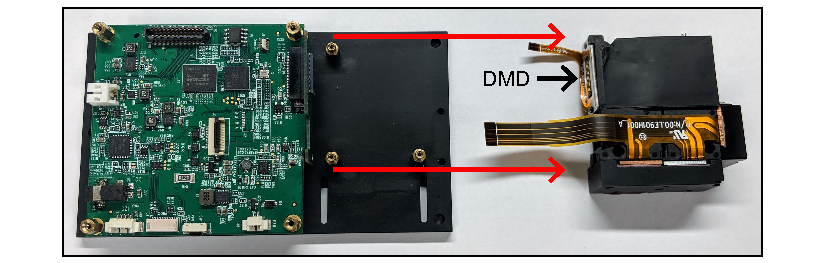
\includegraphics{figures/appendix_b/dmd_mod_4.pdf}
    \caption {
        \label{fig:dmd_mod_4}
        Disconnect the light engine from the board.
    }
\end{figure}

% Figure - LightCrafter Modification: Step 5
\begin{figure}
    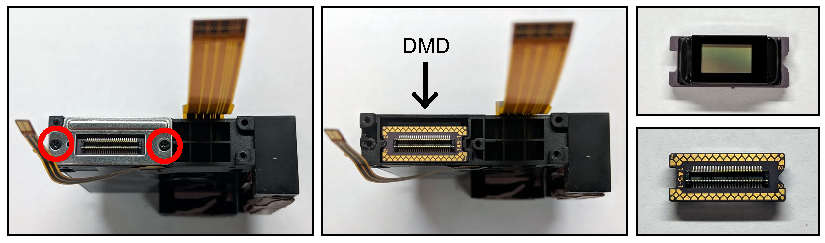
\includegraphics{figures/appendix_b/dmd_mod_5.pdf}
    \caption {
        \label{fig:dmd_mod_5}
        Extract the DMD from the light engine.
    }
\end{figure}

In order to improve physical access to the DMD, the bottom board can be reoriented on the baseplate. Remove the four standoff screws and rotate the bottom board by 180$^\circ$ so that the DMD mounting socket is facing outwards (Figure \ref{fig:dmd_mod_6}). Any modifications to the baseplate (e.g. drilling holes for mounting) should be performed at this stage since all electronics are currently detached. Reattach the bottom circuit board to the baseplate using the standoff screws and reconnect the DMD to its mounting socket. The notch, which indicates the illumination orientation, should be facing towards the right. Reattach the top circuit board and secure with the four screws removed at the beginning.

% Figure - LightCrafter Modification: Step 6
\begin{figure}
    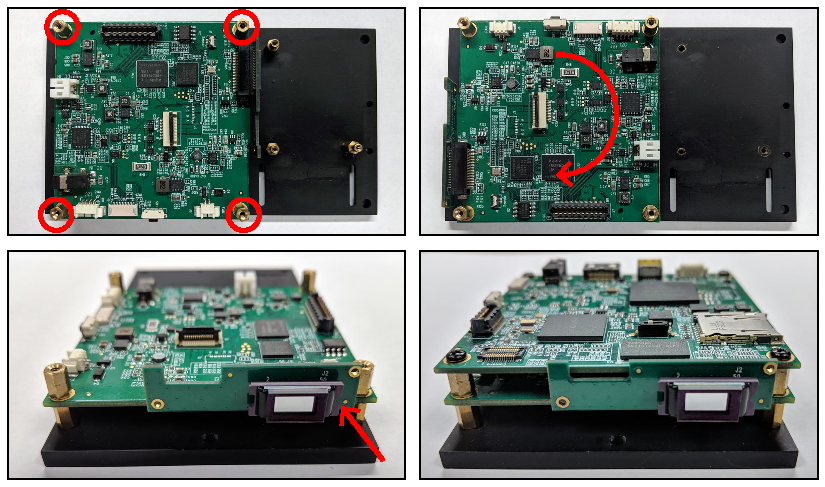
\includegraphics{figures/appendix_b/dmd_mod_6.pdf}
    \caption {
        \label{fig:dmd_mod_6}
        Rotate the bottom circuit board by 180$^\circ$, reconnect the DMD to its socket, and reattach the upper circuit board.
    }
\end{figure}

The LightCrafter is now configured for use with custom illumination paradigms such as the one described in this dissertation. Because the DMD is exposed on the edge of the device, care should be taken to avoid physical contact that might damage the device.



%%%%%%%%%%%%%%%%%%%%%%%%%%%%%%%%%%%%%%%%%%%%%%%%%%%%%%%%%%%%%%%%%%%%%%%%%%%%%%%
% END Appendix B
%%%%%%%%%%%%%%%%%%%%%%%%%%%%%%%%%%%%%%%%%%%%%%%%%%%%%%%%%%%%%%%%%%%%%%%%%%%%%%%
